% THIS IS SIGPROC-SP.TEX - VERSION 3.1
% WORKS WITH V3.2SP OF ACM_PROC_ARTICLE-SP.CLS
% APRIL 2009
%
% It is an example file showing how to use the 'acm_proc_article-sp.cls' V3.2SP
% LaTeX2e document class file for Conference Proceedings submissions.

\documentclass{acm_proc_article-sp}

\begin{document}

\title{uF!t: A Framework for Monitoring Exercises}

% \subtitle{[Extended Abstract]
% \titlenote{A full version of this paper is available as
% \textit{Author's Guide to Preparing ACM SIG Proceedings Using
% \LaTeX$2_\epsilon$\ and BibTeX} at
% \texttt{www.acm.org/eaddress.htm}}}

%
% You need the command \numberofauthors to handle the 'placement
% and alignment' of the authors beneath the title.
%
% For aesthetic reasons, we recommend 'three authors at a time'
% i.e. three 'name/affiliation blocks' be placed beneath the title.
%
% NOTE: You are NOT restricted in how many 'rows' of
% "name/affiliations" may appear. We just ask that you restrict
% the number of 'columns' to three.
%
% Because of the available 'opening page real-estate'
% we ask you to refrain from putting more than six authors
% (two rows with three columns) beneath the article title.
% More than six makes the first-page appear very cluttered indeed.
%
% Use the \alignauthor commands to handle the names
% and affiliations for an 'aesthetic maximum' of six authors.
% Add names, affiliations, addresses for
% the seventh etc. author(s) as the argument for the
% \additionalauthors command.
% These 'additional authors' will be output/set for you
% without further effort on your part as the last section in
% the body of your article BEFORE References or any Appendices.

\numberofauthors{2}

%\author{
% You can go ahead and credit any number of authors here,
% e.g. one 'row of three' or two rows (consisting of one row of three
% and a second row of one, two or three).
%
% The command \alignauthor (no curly braces needed) should
% precede each author name, affiliation/snail-mail address and
% e-mail address. Additionally, tag each line of
% affiliation/address with \affaddr, and tag the
% e-mail address with \email.
%
% 1st. author
% \alignauthor
% Ben Trovato\titlenote{Dr.~Trovato insisted his name be first.}\\
%        \affaddr{Institute for Clarity in Documentation}\\
%        \affaddr{1932 Wallamaloo Lane}\\
%        \affaddr{Wallamaloo, New Zealand}\\
%        \email{trovato@corporation.com}
% % 2nd. author
% \alignauth`or
% G.K.M. Tobin\titlenote{The secretary disavows
% any knowledge of this author's actions.}\\
%        \affaddr{Institute for Clarity in Documentation}\\
%        \affaddr{P.O. Box 1212}\\
%        \affaddr{Dublin, Ohio 43017-6221}\\
%        \email{webmaster@marysville-ohio.com}
% }

\author{
\alignauthor
Brandon Snuggs\\
       \affaddr{Swarthmore College}\\
       \affaddr{500 College Avenue}\\
       \affaddr{Swarthmore, Pennslyvania}\\
       \email{bsnuggs1@swarthmore.edu}
% 2nd. author
\alignauthor
Steven Hwang\\
       \affaddr{Swarthmore College}\\
       \affaddr{500 College Avenue}\\
       \affaddr{Swarthmore, Pennslyvania}\\
       \email{shwang1@swarthmore.edu}
}

\maketitle
\begin{abstract}
Common reasons for the low motivation to exercise include
the absence of an exercise partner and the large time investment
required in traveling to the gym. Some responses to this
issue have divulged possible solutions: joining exercise
support groups or focusing on exercises that can be done without
gym equipment. While both suggestions are practical, 
studies show support groups are notable for being effective
at keeping individuals adherent to a regular exercise routine. 
Furthermore, the modern evolution of social networking sites 
has allowed for support groups to form online. In our current 
iteration of uF!t, we are able to track situps.  Before further 
improvement in the system, we completed an evaluation focused on 
the system's ability to count situps. After establishing that uF!t 
is best placed on either the chest or the side of the chest, we 
were able to retrieve good results from tracking situps.  At the 
moment, uF!t is good at tracking slower speed situps, with slower rate
defined as completing one situp in three seconds or more. From our evaluations, 
we believe that uF!t has great potential to become a system that
can contribute to health exercises including more than just situps.
\end{abstract}

\section{Introduction}
Currently, America's healthcare costs have been rising more 
and more each year. One of the most influencing factors in this
phenomenal increase is due to obesity. In 2008, obesity healthcare
costs account for at least 10\% of total medical expenditures which amount to approximately 
147 million dollars a year \cite{jeffords:obesity}. In addition to the lack of control over how well a patient 
follows drug regiments, doctors cannot guarantee that their patients maintain a regular exercise schedule. 
In a case study involving 20 patients, on the first day all patients agreed that they would maintain their regiment, but after three months, only
seven patients had continued their exercise regiment. In eight months,
only five were consistent with their exercise regiment \cite{campbell:noncompliance}. This case study
reflects the same trend that is present among the general populace joining exercise programs in America. 
Current studies show that 50\% of Americans that join an exercise program will drop
out within the first six months \cite{kravitz:eMotivation}. In order to help the reduction of obesity issues 
medical devices have been created such as body wireless sensor networks that are used to either provide body posture correction/monitoring 
or track daily activities. In many cases, body wireless sensor networks that are used to track an individual's 
activities attempt to motivate users to lead more healthy lifestyles \cite{mulas:race}\cite{ganti:satire}\cite{seeger:healthass}.
The uF!T framework acts as a motivational tool that provides convenient exercise tracking on-the-go. Currently, people
are able to record their exercises by paper or on a spreadsheet.  However, both of these methods are prone to human
error, since it is easy to forget the number of repetitions completed
if not recorded within a reasonable period of time. This predicament is particularly relevant to individuals
completing exercises on the go, where paper or laptop access is not as
easy.  By taking 
out the need to have a gym or time allotted for exercising, an individual would be able to take advantage of 
small pockets of time to exercise. Furthermore, researchers have found that such devices that monitor a person's vitals or exercise information are conducive to leading a healthy lifestyle \cite{acharya:selfmonitor}. Likewise, uF!T intends to assist an individual with a busy lifestyle maintain a healthy lifestyle. With uF!t, we will be able to eliminate the
 hassle of dedicating exercise results to memory and enable users to
  focus more on their workout at any time, thus maximizing the gains from a healthy exercise \cite{acharya:selfmonitor}.

\begin{figure}
\centering
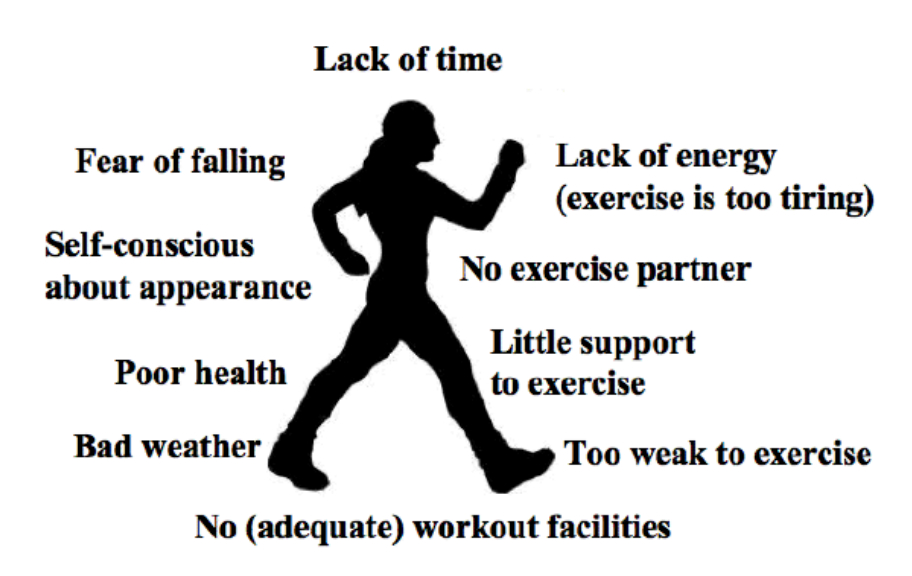
\includegraphics[width=3.0in,width=3in]{./figs/exercise.png}
\caption{Some of the many reasons for not exercising.}
\label{fig:noexercise}
\end{figure}

\subsection{Why don't people exercise?}
While exercise is the main solution to help reducing obesity, people still
choose to not exercise despite the health benefits. This reality may be counter-intuitive for a reason: some
researchers believe that this is due to the increase in fast-paced lifestyles.
In many cases, it is possible to imagine this scenario given the variety of schedules people have to juggle apart from trying to maintain a regular
 exercise schedule (\textit{long work hours, picking
up kids, attending city meetings, taking care of family, etc.}).

A resounding claim among researchers is that the general decrease in exercise in
the US population is is mainly a consequence of technology
replacing usual forms of exercise \cite{jeffords:obesity}. Previously, traversing long
distances were completed by either walking or riding a bicycle; whereas now, such 
distances are covered by either driving or use of public transportation
(which generally involve an individual to be sitting). Following the advancement of technology,
activities that involved physical activity are now being phased out.  Even household activities such as household vacuuming is increasingly replaced by automatons like a Roomba robot.
In addition to fast-paced lifestyles and unavailable schedules, researchers attribute
people's lack of motivation to workout to several different reasons as seen in Figure
\ref{fig:noexercise}. Looking at the figure, we can see that one reason for losing motivation to exercise is 
due to the inability to obtain moral support from a partner or support group.  
It has been proven that people are more inclined to stick to an exercise regiment
if they have a friend or family member that can assist them \cite{plante:exercisewithanother}.
Following what is described in the article by Plante, having an exercise partner
 improves the amount of stress relieved during a regular exercise routine.  Admittedly, we do not 
 believe that uF!t is capable of solving every problem listed in the figure.  However, we 
 believe that uF!t has the possibility of reaching the solution to two problems: \textit{no exercise partner} 
 and \textit{lack of time}.  In the following pages, we will discuss our results about being able to correctly detect peaks from the accelerometer and gyroscope.  Additionally, we will test proper locations for the placement of uF!t to minimize the amount of sensor measurement noise generated by a user's movement.  Lastly, we wish to measure how accurately our system can count situps by doing trial runs with random individuals.  The use of random individuals, we will also allow us to measure if our system is comfortable enough for users of various sizes.  Through an evaluation of the system's current ability to measure situps, we believe that uF!t already has the groundwork that will allow it to track a multitude of various calisthenics.

\begin{figure}[ht]
\centering
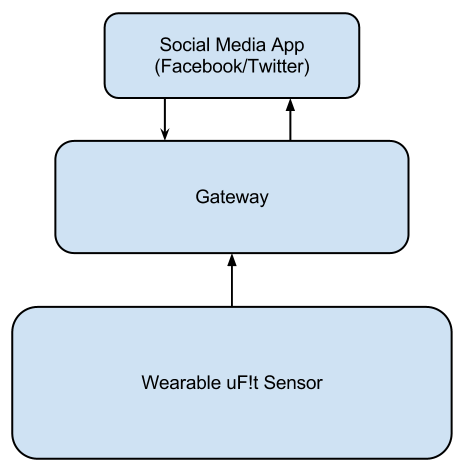
\includegraphics[width=2.0in,width=2in]{./figs/uf!t-system.png}
\caption{An overview of the system we are implementing.}
\label{fig:system}
\end{figure}


\section{SYSTEM ARCHITECTURE}
Our current system only counts situps. Upon the completion of
a situp, if properly detected, uF!T will communicate to a base 
station/gateway (laptop or desktop) wirelessly with a message describing how many situps have been completed so far.  Once the workout has been completed, uF!T would upload the
data to a social media application like Facebook or Twitter; Figure \ref{fig:system} describes the system that we are currently trying to achieve.  Of course, the social media
integration has not yet been implemented, you can find more information on this in the Future Works section.  In this section, however, you will find information about the components about what is currently working in uF!t.

\subsection{Exercise Counter}
The uF!T exercise counter records the number of repetitions completed for an exercise by counting defined features of the exercise. We have specifically defined features for our counter to look for: the counter will 
look for peaks and troughs by filtering sensor measurements through a complementary filter.
In our current iteration, when a user is doing a situp, their body oscillates between two varying angles: the rest
and the peak. Therefore, a rest-peak pair would represent a single repetition of a complete situp.

In order to recognize a peak in the measurement data, such as the angles
found from our situp detector, we set threshold values (i.e. the minimum angle value to be considered a rest
and the maximum angle value to be considered a peak).  Each peak in the measurement
readings is likely to consist of data points that are above the peak 
threshold value and it is common to have multiple data points 
classify as a peak value. The number of successive peak values
indicates confidence that a peak is correctly observed. Typically,
higher frequencies of peak detections in successive measurements would indicate with stronger confidence
that a peak is indeed there while lower frequencies (one or two 
peak detections) might indicate some noise. In order to make our 
system more robust to misclassification due to noise the following conditions must be met before a peak is confirmed as a peak:

\begin{enumerate}
\item \textit{Peak Confidence}: In order to be classified as a peak there must be at least 3 consecutive peak classifications. Otherwise, the classification is assumed to be from noise.
\item \textit{Peak Authenticity}: If a peak is classified recently, another peak classification would be counted toward the recent peak instead of classifying a new peak.
\end{enumerate}

In our current iteration of uF!T, threshold values are chosen by hand. 
In order to account for the potential to have different forms of 
data for individuals, these threshold values will be user-specific.
We hope to gain this information by dynamically updating these 
threshold values and store these in a user profile on the social
media application.

\subsection{Wireless Communication}

Exercise counts are delivered wirelessly to a base station. Once a mote detects the completion of a situp, it will use a broadcast method called identified Best-effort Local Area Broadcast (libraries provided by Contiki 2.6). Messages that are sent to the base station are received through another mote connected to the base station. We chose to implement wireless communication as mote-to-mote communication because of the simplicity of construction. The structure of wireless communication code on both motes are basically identical. 

Overall, the Best-effort broadcast will periodically broadcast about a completed situp until it receives an acknowledgment from the receiving end.  Included in each broadcast message is a header that identifies the sender and the receiver is hard-coded with the address of the sender such that only messages sent from the specific sender will be accepted.  Implicit in this form of wireless communication we have accounted for mote security and data reliability. The base station will not falsely count additional situps for other nearby motes that may also broadcast completed exercises. 

\section{Implementation}
We used the Tmote Sky for the basis of our project. The Tmote 
Sky can be powered by two AA batteries for wireless communication. Besides the electrical components, we have encased our
device using a lightweight plastic container (similar to a soap bar case).
The housing for our device helps the sensor sit in a stable position.
The sampling measurement data from sensors are already noisy, so it is important that the sensors are not
given more opportunities to be mutated by noises induced by the sensor
rocking carelessly.

To secure the device around a user's body, we have attached a neoprene
corset to the uF!t's casing (see Figure \ref{fig:devicecase}).  The elastic qualities of the neoprene
corset allows us to secure the device around big as well as small
bodies.  This versatility has allowed us to further reduce any noise
produced from rocking the sensor and it has proven to be comfortable
as seen in our evaluations.

\begin{figure}[ht]
\centering
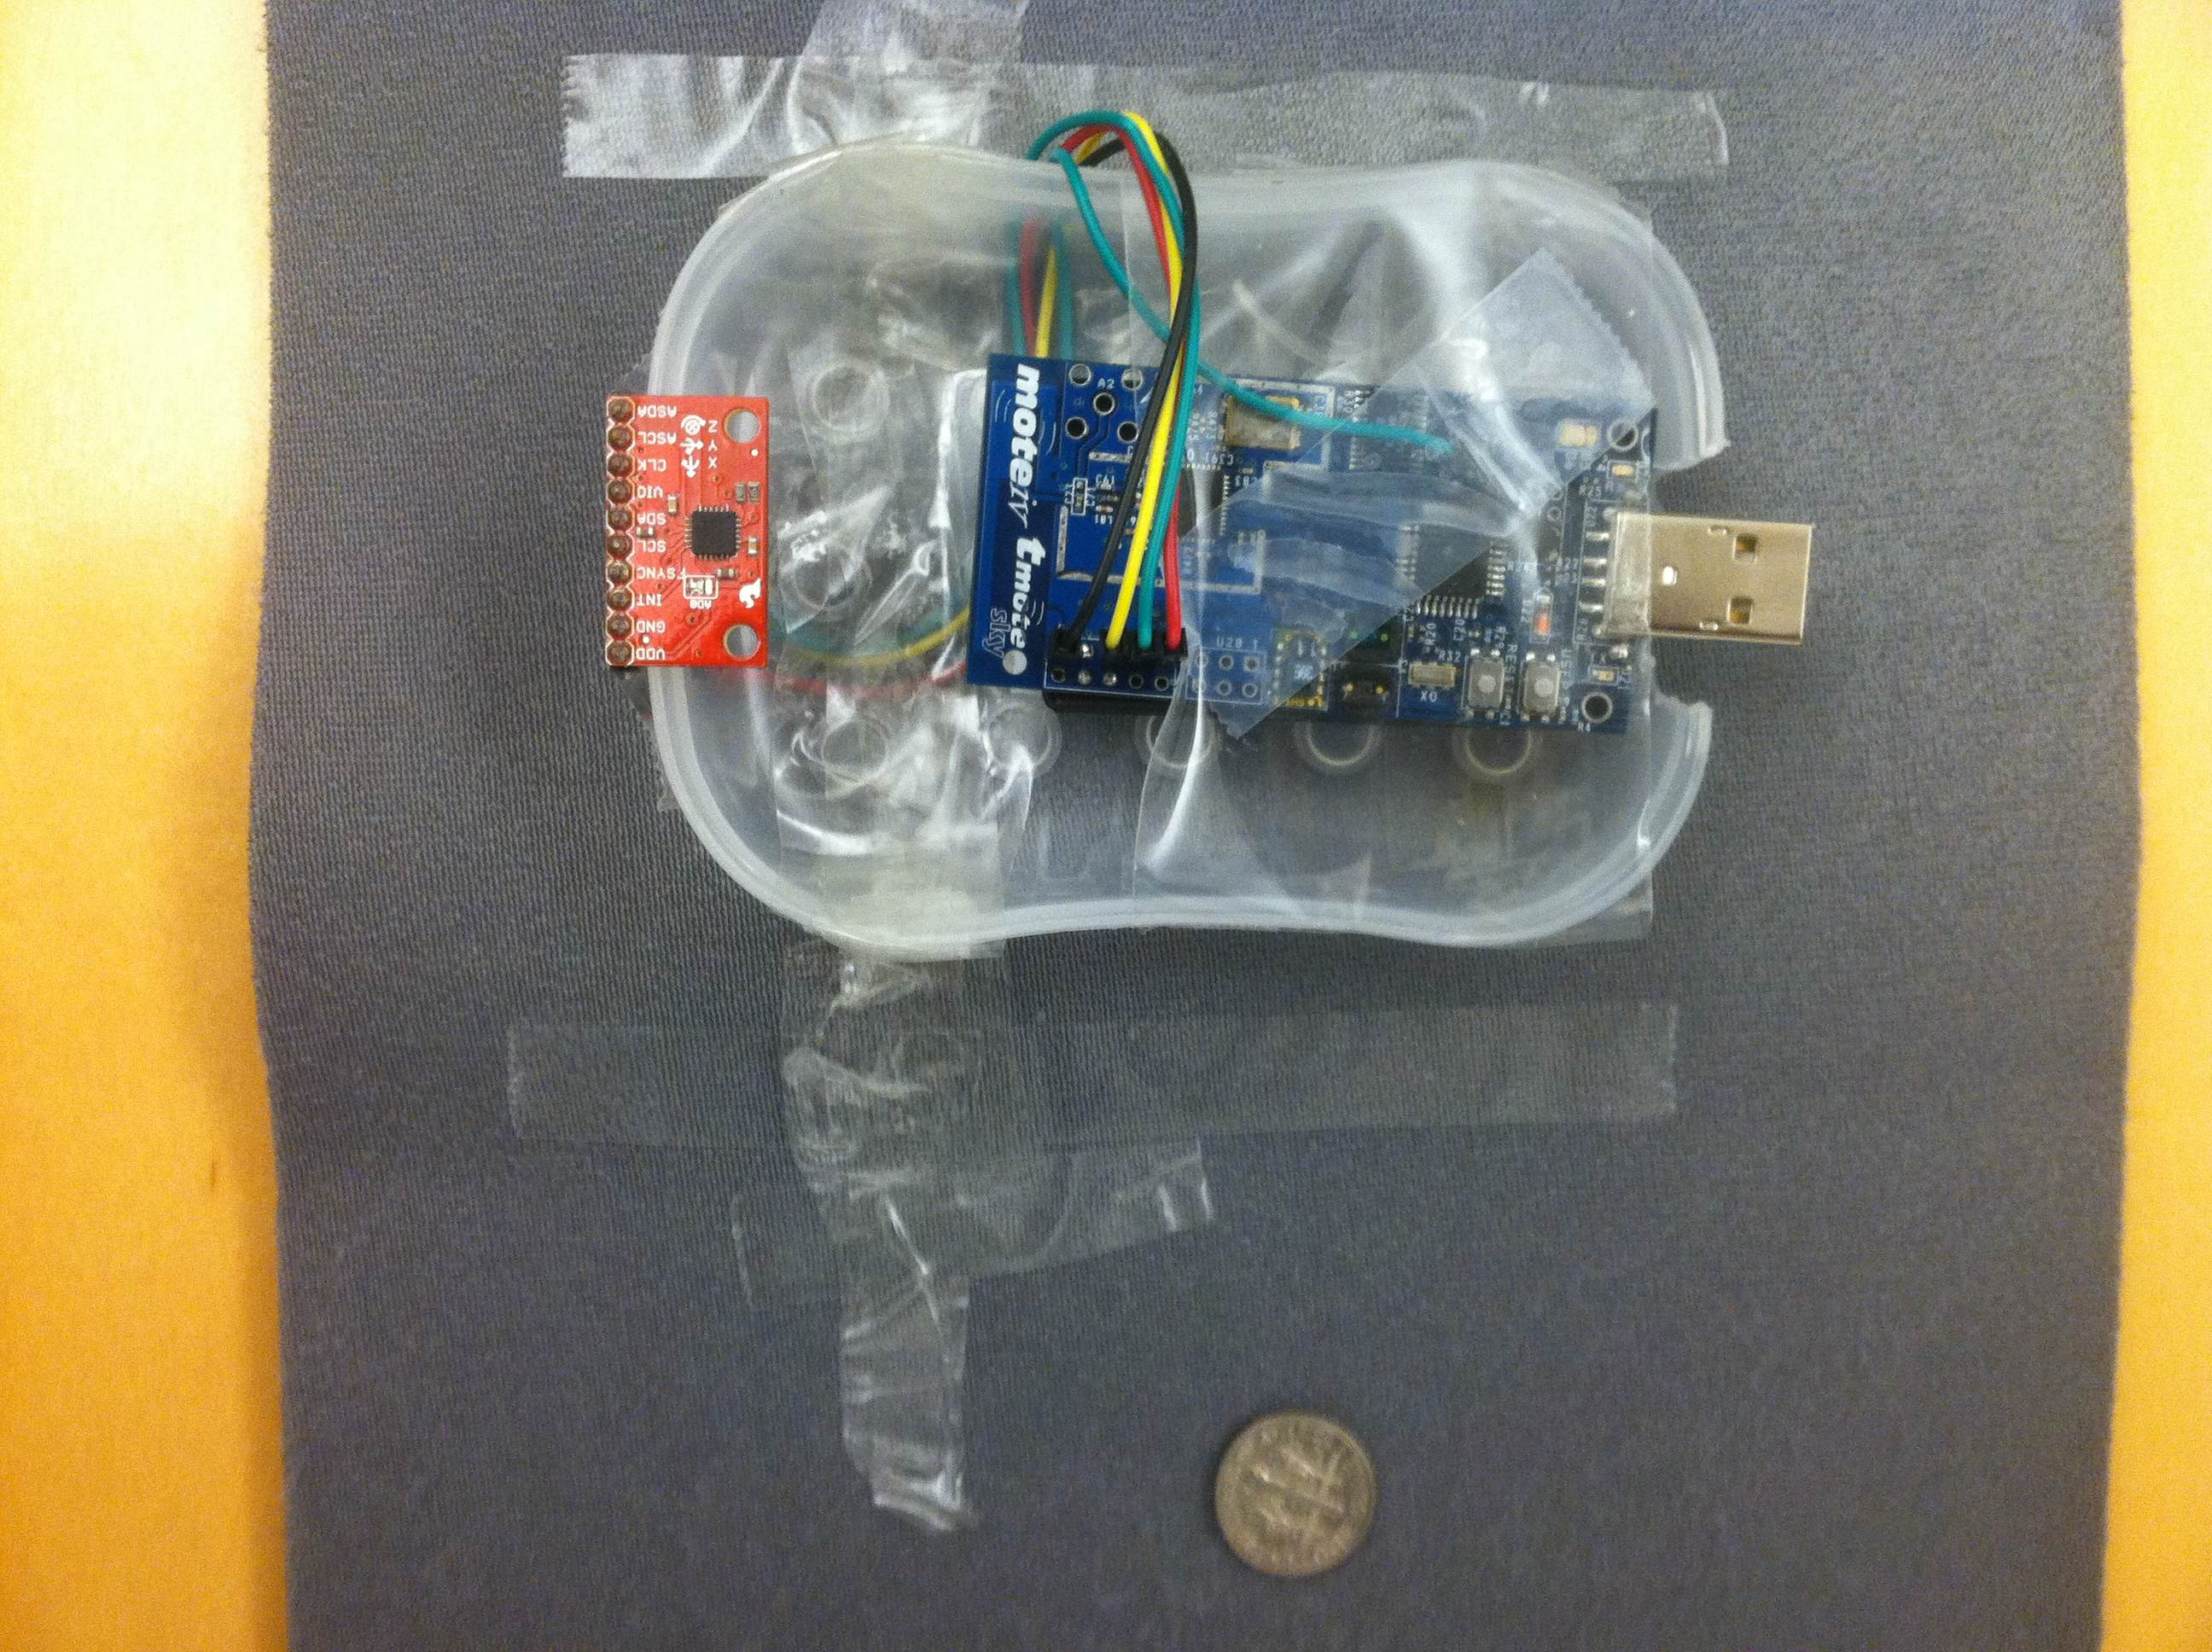
\includegraphics[width=2.0in,width=2in]{./figs/tmote-size.jpg}
\caption{The current casing for our uF!t device, size compared to a dime.}
\label{fig:devicecase}
\end{figure}

\subsection{Software: Contiki 2.6}
Unlike a standard out-of-the-box Tmote Sky, we used Contiki 2.6, instead of
using TinyOs.  We chose to make this decision since our team was much
more familiar with C, which made it much easy for us to quickly
understand native functions in Contiki 2.6.  This allowed
us to focus on understanding how to integrate the accelerometer and
gyroscope's functionality into Contiki. Furthermore, because of the limitations of Contiki's math library in the design our program we found lightweight approximations of some necessary math functions for our own use (the authors of that atan2 function that is used is cited in the code).

\subsection{Hardware: mpu6050}
We have connected the 3-axis Gyro/Accelerometer mpu6050.  The gyroscope
contains various degrees of sensitivity, which can be easily
modified with Contiki functions that we have created. The mpu6050 sensor
also contained a temperature gauge; for the time being, we did not 
incorporate the temperature gauge into our project, but we believe it may
have later uses in different exercise regimens (for more info please look at future works).

To ensure that we could track a user's body while doing a situp,
this required more work than just using the accelerometer and 
gyroscope raw data.  As such, we ran through
some equations that either used the accelerometer or the gyroscope.
However, after running some tests separately on the accelerometer and
gyroscope, we decided that we would need to use the measurements received
from both devices in order to calculate the angle of user's body.

\begin{figure}[ht]
\centering
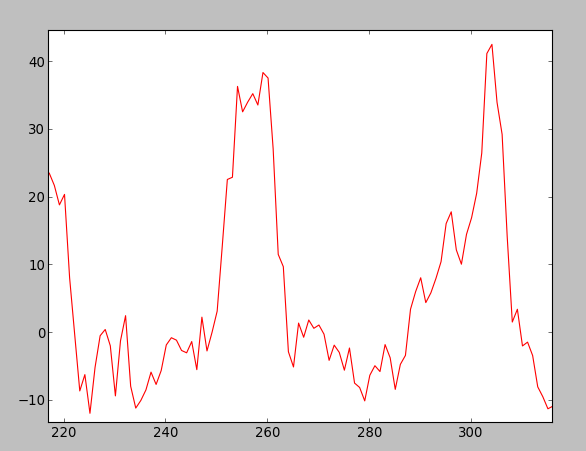
\includegraphics[width=3.2in,width=3.2in]{./figs/accel_test.png}
\caption{The results of the accelerometer.}
\label{fig:accelResults}
\end{figure}

\subsection{Accelerometer}
In order to track simple movements like a push-up or sit-up,
we focused on variation in the 
accelerometer's z (for the push-up) and the accelerometer's
y (for a pull-up).  However, calculating the angle
of the user's body with respect to our sensor requires some
trigonometry involving the accelerometer data.

\begin{equation}angle_{accel_x} = \arctan(accel_x,accel_z) + \pi\end{equation}

Using the equation above allows us to calculate the tilt angle 
for the accelerometer. Arctan, outputs between the range of \(-\pi\) and \(\pi\), so you
must add \(\pi\) to the results of arctan to have the range converted
 to 0 to 2\(\pi\).  Having no initial knowledge in the usage
of accelerometers or gyroscopes, we believed that the accelerometer
 would have served its purpose for calculating the wearer's
body angle during a situp.  However, if we look at Figure \ref{fig:accelResults}
we can see that our initial assumption was clearly untrue.  The
accelerometer is great at calculating angles for stationary 
positions, but it is terrible at tracking the rapid movements 
experienced during a situp.  After doing a real-time comparison
of an actual situp and the data we recorded, it turns out that
the accelerometer reports angles exceedingly lower than what is
actually completed.  In our initial tests, we only did situps
up to angle of \(60^\circ\), however when we look at figure \ref{fig:accelResults},
we can see that the highest recorded peak is about \(40^\circ\).  Additionally,
the data that we received was noisy, so this was unsuitable for
accurately tracking a user's angle.

\subsection{Gyroscope}
The gyroscope is able to calculate angular velocity in degrees 
per second, which lead us to think that the gyroscope would
provide more promising results (we would use a discretized time model to update the current angle). Therefore, angle accuracy would be solely dependent on the fidelity of the gyroscope measurements. For the gyroscope, we used 
this simple equation to calculate the angle.

\begin{equation}angle_{gyro_x} = angle_{gyro_x} + gyro_x*dt\end{equation}

Gyro is the degrees per second (\(^\circ/s\)) recorded from the
gyroscope, while \textit{dt} is the sample period calculated from 
the sample speed.  
Multiplying the gyro by sample period, gives us the angle calculated 
within one cycle, which can be accumulated in our total angle.  
Successfully being able to calculate the angle using the gyro, 
we were certain that our results would be promising.  Looking
at figure \ref{fig:gyroResults}, however, the gyroscope's measurements are 
constantly increasing by a fixed amount as time goes on, this
is called \textit{drift} which is typically an issue in most gyroscopes.  From our gryoscope analysis, our
gyroscope not only experiences bad drift (about \(5^\circ/s\)),
but it also is not centered properly.  Currently, when the gyroscope is
stationary, it returns an angular velocity of \(34^\circ/s\)
in motion.

\begin{figure}
\centering
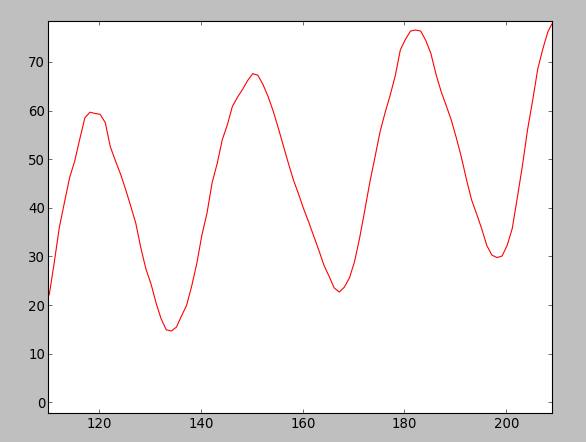
\includegraphics[width=3.0in,width=3in]{./figs/gyro_test.png}
\caption{The results of the gyroscope, smoother than the
accelerometer results.}
\label{fig:gyroResults}
\end{figure}


\subsection{Complimentary Filter}
From our analysis, we can see that both accelerometers and 
gyroscopes have pros and cons.  The accelerometer 
is good at detecting static positions; however, whenever
the sensor is moving very quickly, it returns very noisy data.  In 
contrast, the gyroscope is good at detecting rapid 
movements, however its data drifts over time, making it 
increasingly inaccurate the longer you monitor the gyroscope.

The solution involves using a combination of the
accelerometer and gyroscope data.  After researching sensor filtering techniques we found that some filters
involving body movement detection utilized either the Kalman Filter or other variations of it (Extended Kalman Filter, Fast Kalman Filter, etc.).  However, in our research we were not able to find any articles
about utilizing the Complimentary Filter to analyze data.  Since
the Complimentary Filter is computationally cheaper than the Kalman Filter, we decided to begin our research here \cite{colton:filter}.

\begin{equation}angle_x = (a)*(angle_x+gyro_x*dt)+(1-a)*(angle_{accel_x})\end{equation}

With the knowledge that we cannot rely on the gyroscope for 
long periods of time, it is important to calculate a good time
constant.  The time constant \(\tau\) helps determine the coefficients (\textit{a} and 1-\textit{a}) used in the filter.

\begin{equation}\tau = \frac{a*dt}{1-a}\end{equation}

The time constant \(\tau\) may vary from user to user depending on
the reliability of the gyroscope's data and the sample
rate.  The time constant defines the boundary between
trusting the gyroscope and trusting the accelerometer.
In our time constant, we used a time constant of \(\tau\)=\textit{0.5
seconds}. We had chose this time constant due to our results
from the gyroscope (it is important to choose a time constant
that will work with the amount of drift generated from the
gyroscope).  This means that for any measurement that is
lower than half a second, the algorithm will weight the
gyroscope's measurements more heavily.  However,
for any measurements that take longer than half a second,
the accelerometer measurements will have more weight over those of the gyroscope.  Since the gyroscope drifts over time, under shorts periods of time (such as a quick rise during a situp) measurements are
very reliable.  However, consider a user
that has already risen and is waiting at the peak of their
situp.  In this situation, the gyroscope will become
unreliable as time continues to expire, so it is better
to trust the accelerometer's data because it is suited
for recording angles in stationary positions.  Using the
complementary filter in this style, we would be able to record situps at varying speeds by minimizing the error-prone effects of each sensor and maximize the utilization of their advantages.


\section{Evaluation}
In order to estimate how well our uF!t system is working, it
will require the evaluation of two things: Peak Detection algorithm
and Sensor Placement. Evaluation of our Peak Detection algorithm is essential in the process of determining if uF!T is able to correctly
detect a situp.  Poor recognition of a simple situp
would introduce cascading errors for our system when we attempt distinguish a situp from other exercises. We chose to test Proper Sensor Placement in order to determine in what ways the mote would be adversely affected by the  sensor shifting. By placing uFit in "shifted" areas, we would simulate real-world scenarios in which the data may suffer from additional unwanted 
noise.

\subsection{Peak Detection}
There are two important terms that we use for our Peak
Detection algorithm (as described briefly in Section 3.1): \textit{peaks} and \textit{rests}.
Peaks occur when the user has effectively slowed
their angular velocity to 0, while also being above a
threshold value.  Rests are the complete opposite, they
are moments when the user's angular velocity is close to 0,
while also being below a threshold value.  In our current 
implementation, we have designated zones to represent "good"
areas for peaks and "good" areas for rests.  These "good" areas
are set by threshold values that have been determined based upon monitoring other people who were doing situps. An angle of \(50^\circ\) or higher represents the
threshold value for peaks, while \(10^\circ\) or below
represents the threshold value for rests. Statically defining threshold values is inflexible when detecting situps given that an individual is likely to vary their situp form.  However, initially choosing static threshold values provided
us a quick and simple way to begin detecting situps without
having to use anything that is more complex.  Looking
at Figures \ref{fig:centerchest}, \ref{fig:sidechest}, and \ref{fig:sidearm}, 
we already have results from the threshold values that we selected.
The upper blue dots, represents detected peaks, while the lower green
dots represent detected rests. Like our competitors, we too have provided
in-sensor calculations, allowing us to minimize the amount of data that
will be sent wirelessly.


\begin{figure}[!ht]
\centering
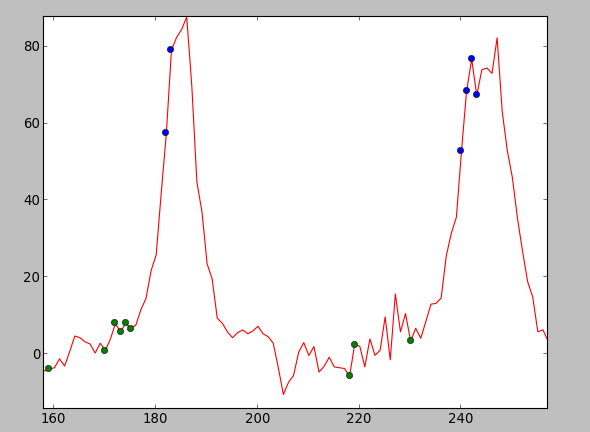
\includegraphics[width=3.0in,width=3in]{./figs/chestTestcenter.png}
\caption{The results of the complimentary filter with sensor placed
on the center of the chest.}
\label{fig:centerchest}
\end{figure}

\begin{figure}[!ht]
\centering
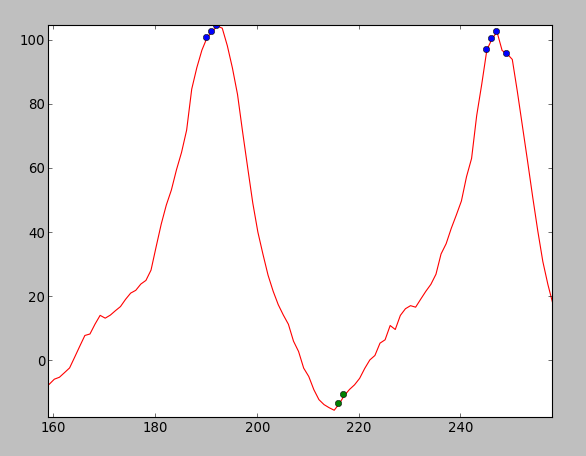
\includegraphics[width=3.0in,width=3in]{./figs/chestTestside.png}
\caption{The results of the complimentary filter with sensor placed
on the side of the chest.}
\label{fig:sidechest}
\end{figure}

\subsection{Proper Sensor Placement}
For testing proper sensor placement, we tested several
areas where the sensor could be placed on a user's body.
As stated earlier, it is important to choose a good location for the 
system since it may affect the overall quality of the data.  Additionally, we must consider whether
or not the placement of the sensor is comfortable for
the user.  In our preliminary tests, it seems that it was
acceptable to place the device on the following three
places: \textit{the arm, center of the chest, and the side 
of the chest.} We assumed that the center of the chest
would provide us with the most accurate data, since it
is centered at the body and it should not affect any of
the data since the chest area is generally an even area
for people of most sizes.

Looking at the graphs depicted in Figures \ref{fig:centerchest}, \ref{fig:sidechest}, and \ref{fig:sidearm}, we see that
our initial assumption was actually incorrect.  It seems
that the sensor obtained the best results when it was
placed on the side of the chest (Note how in the snapshot the data representing the motion is smoother than in the other two graphs). We currently do not have an explanation for this occurrence and it warrants further investigation. Of course, we expected
that the arm would not be the best place since depending
on the user, they may either do a situp with their arms
placed on the side of their body, or they may do it with
their arms crossed across their chest. 

These results were nice for our initial attempts, however,
we believe that it lacks the diversity of different sized
bodies for the test results.  We believe that if we can
get more people for our analysis, we can see if the positions
that we have provided are universally good for different
sized people.  So far our preliminary results have been
tested on average-sized males, which currently is a limited
scope of view considering that we wish this device to be
used by many people.

\begin{figure}[!ht]
\centering
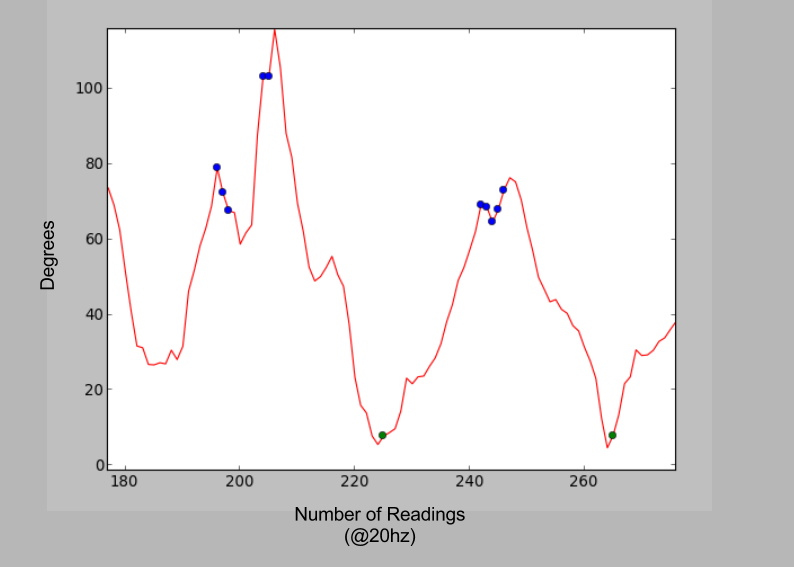
\includegraphics[width=3.0in,width=3in]{./figs/armTest.png}
\caption{The results of the complimentary filter with sensor placed
on the arm.}
\label{fig:sidearm}
\end{figure}

\subsection{Situp Count Accuracy}
Remembering the last section, we determined that it
is important that we are able to detect the correct amount
situps with individuals of varying body types.  For our next
tests, we used four random individuals to do situps while
wearing our uF!t device.  Each user was properly informed
about what our device is capable of and they were given the
choice to decline.  Our test comprised of
three different situp speeds: \textit{fast, normal,} and
\textit{slow}.  Fast is equivalent to completing a situp every
second, while normal is completing a situp every two seconds
and slow is completing a situp every three seconds.  Each individual completed ten situps at each speed.

To ensure that each set of situps was completed in the same
fashion, participants were given a 10 minute break to allow
them to recuperate if they were feeling fatigued.  Determining
the accuracy of each set of situps involving the comparison between
the amount of situps that uF!t detected and the amount situps
counted.  As stated earlier, the stress of workout can impact
a person's ability to record situps.  To avoid the human error
of our participants, we allowed third parties to count the
amount of situps being done for each subject.

For our sampling speed, we chose 20hz for our measurements.  As seen in some related
works, there have been tests using higher sampling speeds to
record data \cite{farringdon:sensorbadge}.  However, when reading
about the SATIRE device, their group was able to achieve decent
readings with using only 25hz \cite{ganti:satire}.  In accordance with our
future works for uF!t, we wish our device to be usable on the go.
We will not be able to accomplish this goal if our device consumes
too much energy. Higher sampling speeds means that our device will
have higher power consumption.  In our initial design of uF!t,
we found that 20hz was the lowest sampling speed possible while
still producing reasonable results; lower sampling speeds were unable 
to keep up with the slowest situp speed.



If we look at the table 1, it seems that our device is highly accurate
when the user is utilizing a slow situp speed (average of .7875).  Unfortunately,
as the user completes sit-ups at a normal speed, the device's accuracy
drops by a factor of 1.88 (average of .425).  This accuracy drops even
further when the user is completing situps at a fast speed, dropping
by a factor of 5.3 when compared to the slow situp speed (average of .15).  



\subsubsection{Participant's Comments}
Considering that we intend uF!t to be used by different people, it is
important to record our participants initial thoughts about our device.
After the completion of the test, each participant was allowed to see
the results of their situps and were asked a small questionnaire with the
following questions:

\begin{table*}[!htp]
\centering
\caption{Accuracy of Situps}
\begin{tabular}{|c|c|c|c|} \hline
Participants&Accuracy (Slow)&Accuracy(Normal) & Accuracy(Fast)\\ \hline
1 & .8 & .4 & .2\\ \hline
2 & .9 & .7 & .1\\ \hline
3 & .5 & .1 & .1\\ \hline
4 & .8 & .5 & .2\\ \hline
5 & .7 & .5 & .2\\ \hline
6 & .9 & .4 & .1\\ \hline
7 & .8 & .5 & .1\\ \hline
8 & .9 & .3 & .2\\ \hline
Average & .7875 & .425 & .15\\ \hline
\end{tabular}
\end{table*}

\begin{figure}
\centering
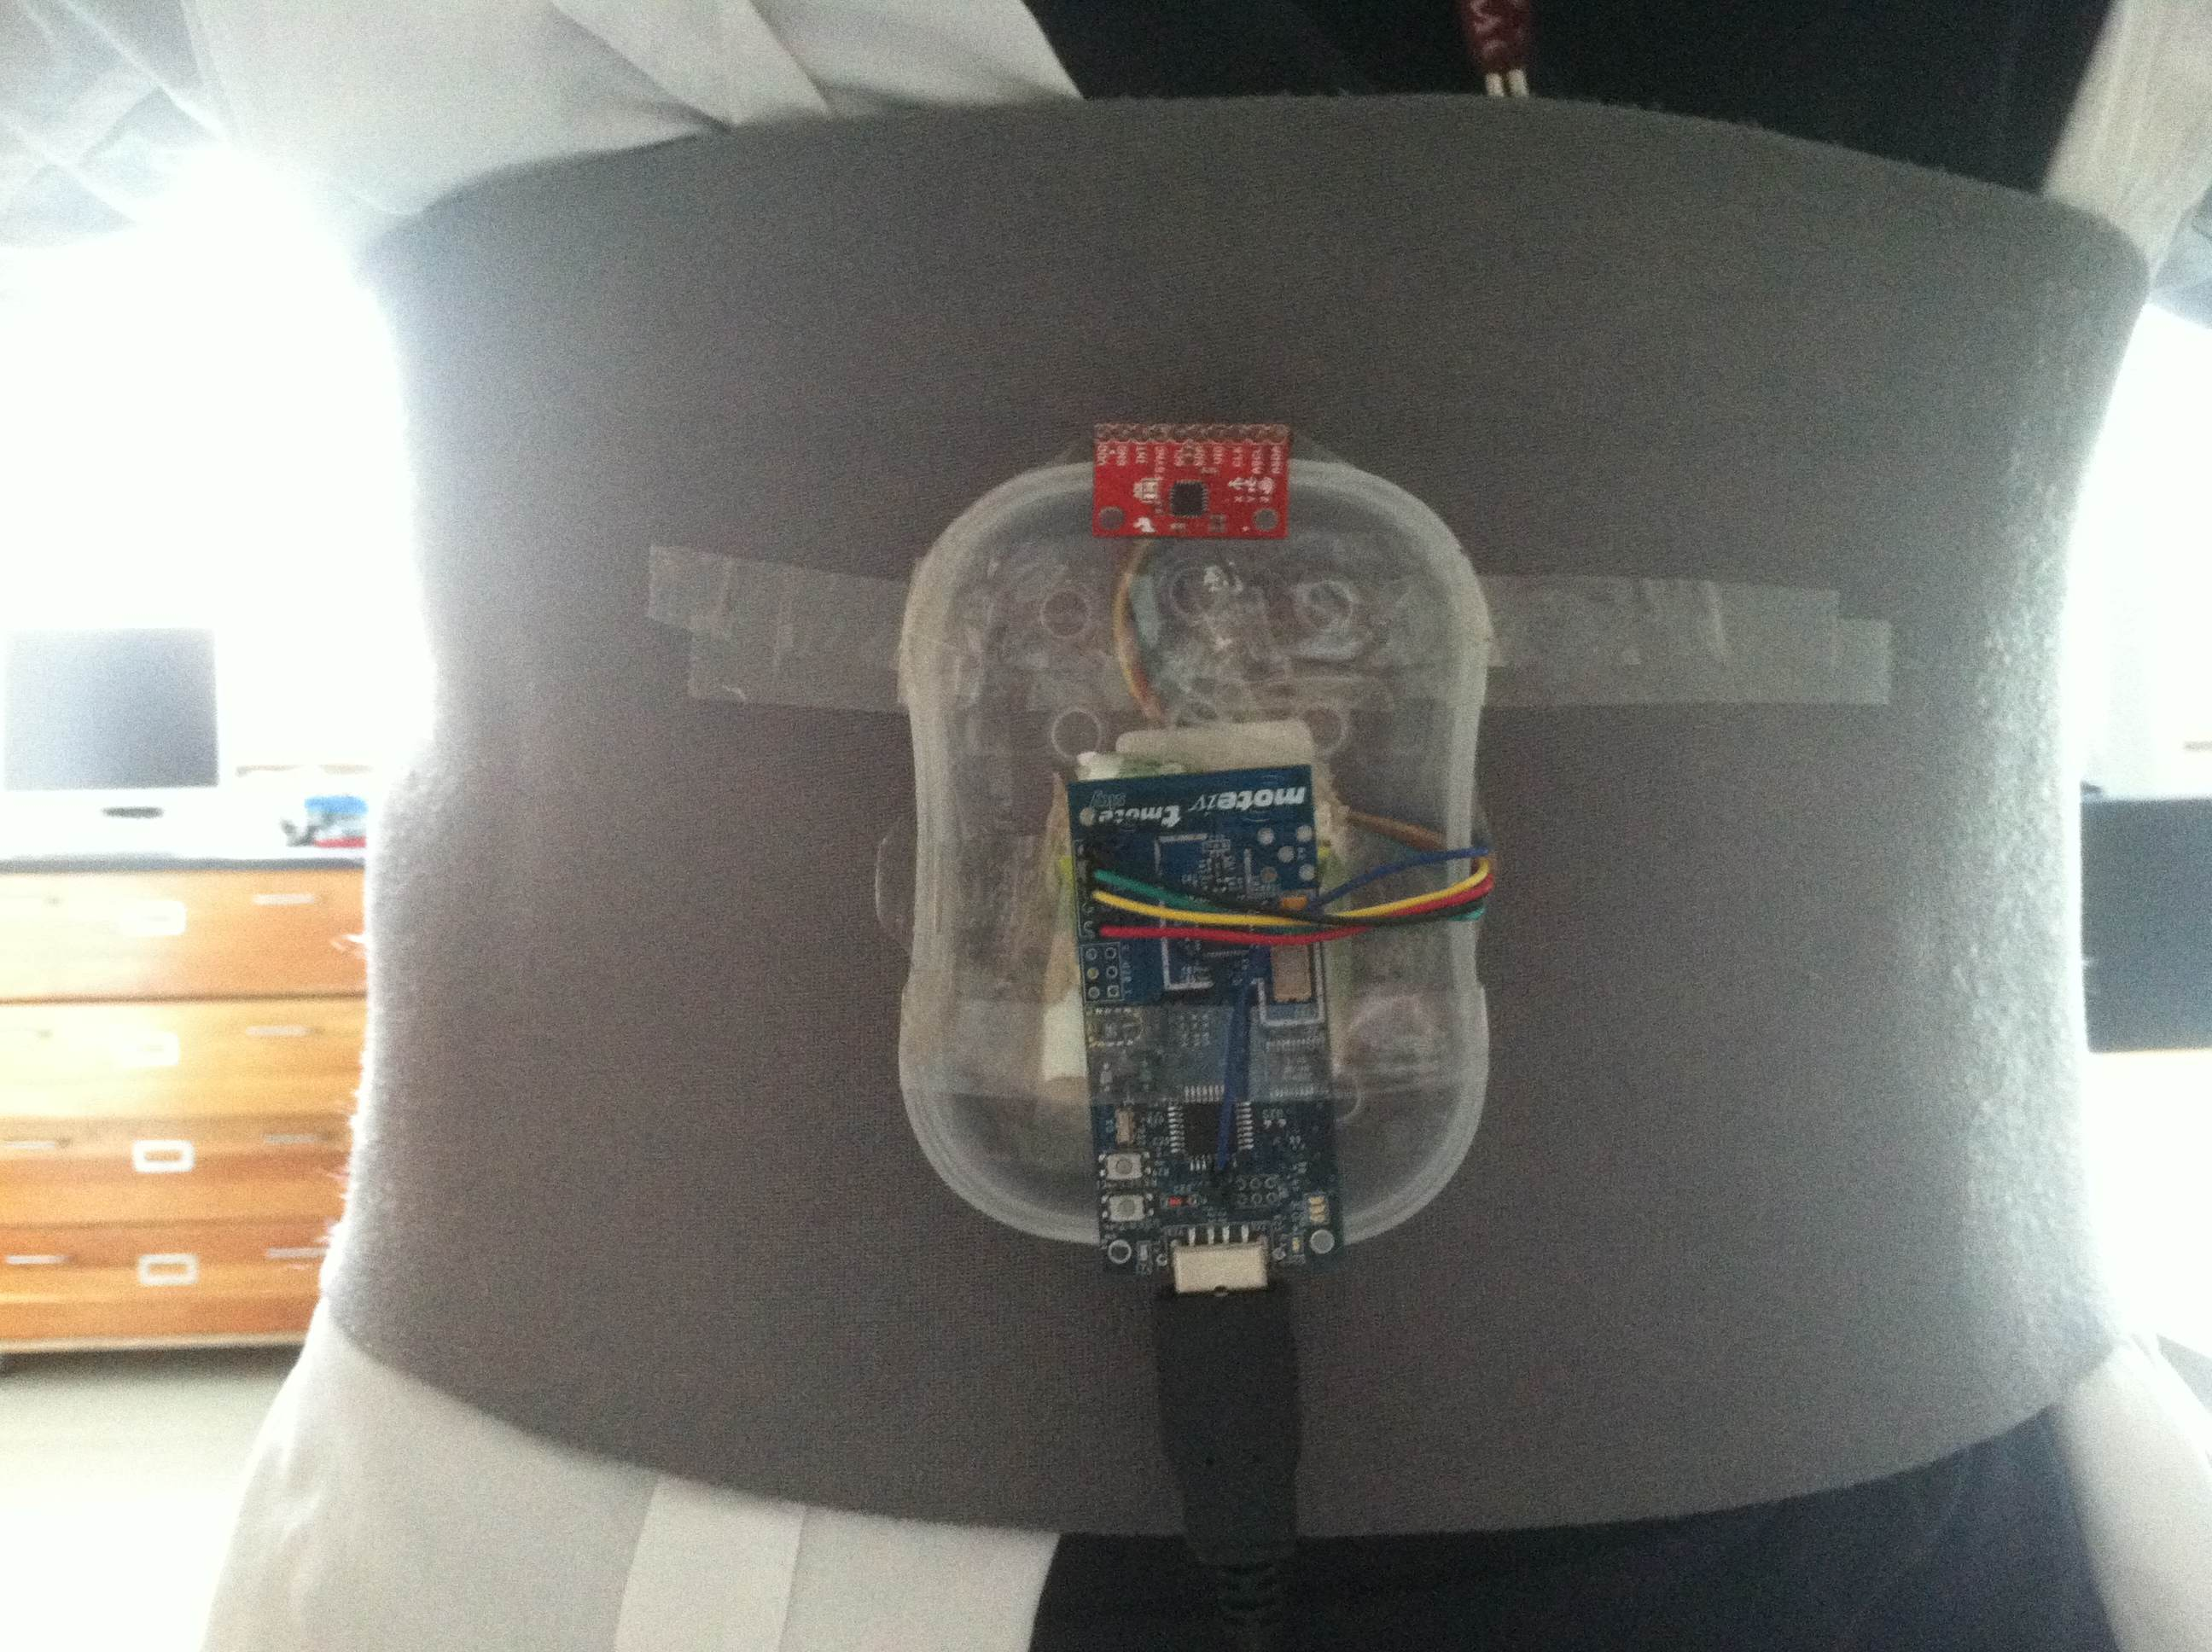
\includegraphics[width=2.0in,width=2in]{./figs/tmote-worn.jpg}
\caption{Example of participant wearing uF!t device.}
\label{fig:deviceworn}
\end{figure}

\begin{enumerate}
\item Do you consider yourself a casual or hardcore exerciser?
\item Did you like using the uF!t device? Was it comfortable?
\item Any additional comments?
\end{enumerate}

Out of the eight test subjects, five identified
themselves as casual exercisers saying that they enjoyed that the
device was able to track their situps when they were completing a
slow set.  However, the other three participants that classified as 
hardcore did not appreciate that the device was unable to detect
a fast set of situps.  The hardcore exercisers said that they needed
to do a larger quantity of faster situps to reap any benefits.
Some participants commented that the important part of
recording the situp is the rise.  This confirms some of our observations
during the tests where a participant's situp would not be detected until
a proper rest-peak pair was confirmed on the situp device. There were also
comments about the device still being comfortable, despite it being
worn by participants of vary sizes.  As we described in Proper Sensor Placement,
it is important to gauge the comfortability of doing the situps with the device,
since its placement can provide unnecessary noise into our data sets.


\section{Related Works}
Unlike uF!t's use of the accelerometer and gyroscope, one of our
main competitors rely on the raw measurements received from using only 3-axis accelerometers 
\cite{seeger:healthass} .  However, unlike
our design, they use multiple accelerometers.  This allows their
system to have more versatility than the amount of exercises that
we are attempting to track.  So far, our exercises are limited to
calisthenics, whereas myHealthAssistant is able to track resistance and 
weight training exercises.  The ability to do more of these
exercises come at a cost.  In their paper they do not cover the
amount of power consumed by using multiple sensors.  This can
make or break the effectiveness of myHealthAssistant
since it is not useful to record multiple exercises with only
a short amount of battery life.  In our current design, we admit
that we have not provided results for uF!t's battery life too.  However,
we have not reached the phase where we can focus on analyzing
uF!t's battery life.  For these reasons, we make note of myHealthAssistant's
lack of battery life discussion because it is important reminder for a device
that is marketed to be used by people that are on the go.

SATIRE is another system that rivals some of the functionalities
that uF!t provides. In SATIRE, they create a body sensor network that is
integrated into a simple winter coat \cite{ganti:satire}.  Their work is related to
uF!t since the system they create involves determining the activity
being performed by the wearer.  They use simple actions such as
walking, sitting, climbing stairs, typing, and reading.  To monitor
these actions they use an \textit{exponential weighted moving average}
(EWMA) filter.  We find this paper very
interesting, since they use it as a way to figure out basic repetitive
actions (they provide 4 labels: stillness, typing, walking, fall).  With
the uF!t device, instead of monitoring day to day activities like SATIRE,
we wish to focus on calisthenic exercises.  Even though SATIRE is only 
for tracking normal activities, it allows them to maintain records on
the wearer's health.  uF!t provides flexibility, considering that it is
not only good for maintaining the user's health, but useful for improving
one's health as well.  Our uF!t device, once fully completed, can be
used for people and patients who wish to be healthier through doing
simple calisthenics.  As stated before, uF!t will be able to track
your progress by storing results from daily workouts, whereas SATIRE
is not necessarily an exercise device, but only a device that
monitors your current health and activity. Similar to SATIRE, we have found other researchers who have attempted specific movement recognition.  The system provided by John Varkey et al, focused on classifying different movements, such as the following: standing, walking, smoking, jogging, and writing \cite{varkey:human}.  Unlike SATIRE, however, they used a machine learning approach by implementing
a support vector machine (SVM), to recognize the different activities.
Although their results are not useful to the current iteration of
uF!t, we believe their research will be conducive to our efforts to
recognize different calisthenic exercises.

Wireless Body Area Network (WBAN), is another device that has
gait/motion detection \cite{jovanov:wban}. However, WBAN, unlike the other research we found, is capable of measuring your "fitness level" while exercising.
Beyond the accelerometer for gait detection, WBAN has several
additional components such as: Temperature/Humidity monitor, Electrocardiogram sensor, motion sensors, and SpO2 (Oximeter).  Following a model similar to ours, WBAN can forward this information
to a gateway, which in their case is a PDA.  From the PDA, the information is forwarded to various servers, which can either be a medical official's server, your home computer, or your emergency contact's computer.

Many mobile application developers have sought to provide creative solutions that complement 
a packed schedule and low interest in exercising. Mobile 
devices such as smartphones, ipods, and chips built into shoes now
are equipped with considerable computational power and are very
portable. Some notable examples of mobile devices are as follows: Nike fit (an ipod 
application that is available on most ipod devices) is available
on many Ipod devices as an application that encourages users to
run by logging the distance run, calories burned and time of an
individual's runs. Another application is \textit{Zombies, Run!} which has 
sought to encourage individuals to exercise by introduce a gaming
aspect to the routine as well as the ability to share results via
social media. The \textit{Zombies, Run!} application has shown to be successful
by popular account and has therefore involved encouraged many people
to exercise more \cite{sixtostart:zrun}. Unfortunately, the \textit{Zombies, Run!} application is extremely
limited in its variety exercises. Researchers believe that there is some correlation between
exercising and social media applications.  There are plenty of benefits, such as increased motivation for exercise, but there also drawbacks, such as increased sedentary behavior from staying connected to the network instead of exercising \cite{vickey:twitterstudy,vickey:fitnesstwitter}.  As seen with \textit{Everywhere Race!}, they also believe that you can promote better health through the use of
famous social networking applications \cite{mulas:race, bausch:framework}. In \textit{Everywhere Race!}, people were allowed to connect with other users in a virtual run.  This virtual run would allow multiple connected users to run a specified distance in different locations while still being able to compete in a virtual race with each other.  However, all of these fitness apps share one thing in common: they only measure running data; as explained, \textit{Zombies, Run!} and \textit{Everywhere Race!} is only capable of encouraging a user to run; furthermore, the researchers data did not involve applications that do more than just tracking running exercise data.  UF!t offers a variety exercises, so that
a user will not have to stick to the same routine.  Being able to change
your routine has been proven to provide better health benefits, than
a routine that is always the same.


\section{Future Works}
Currently, UF!T is limited in its capabilities to provide portable exercise tracking and counting.
However, in order to extend the number of features available to its users, we plan
to add functionality using the temperature sensor, a workout classifier and dynamic
peak detection.

As stated earlier, the mpu6050 contains a temperature sensor.  In
future designs of uF!t, we believe that we can incorporate the
temperature sensor to monitor the amount of heat being generated
during a workout session.  With this data, we want to be able
to determine if the user has been working out for too long.  This
would be idealistic for situations where the wearer is exercising
in undesirable conditions, such as a small stuffy room.  Given
our initial research, we believe that by monitoring the temperature,
we can prevent uF!t users from suffering from severe illnesses such
as dehydration and hypothermia \cite{gonzalez:exerciseheat}.  For those mindful of safety, this feature would be enticing for new people who are interested
in exercising.

\subsection{Workout Classifier}
We intend uF!T to interpret accelerometer and gryoscope data in order
to determine what exercise is being performed. Sensors measurements
would include angular velocity around each axis and 
acceleration along each axis and be stored in a 6-tuple. The
k-means classification algorithm would be used to group these measurements into 
motion features such as movements around the principle axis (i.e. yaw for gyroscope 
and thrust for accelerometer movements) which would consequently be grouped into clusters which 
assist our exercise classifier. Each exercise would be described by a series of clusters.
For example, a situp would consist of clusters describing the positive and negative pitch rotations
based off positive gyroscope values. As an exercise is being conducted, we would provide
templates for each exercise in order to serve as a comparison. Each template would
provide the coordinates of the cluster centers that describe an exercise.

We note that we have not classified the characteristics of many exercises
besides a situp. Furthermore, it is possible to have an individual
do an exercise that is currently not defined. In this case, this
exercise would be classified as an unknown exercise and still be
tracked and counted. For each unknown exercise, the user would be given 
the option of specifying a name for this exercise so that it could be 
tracked in the future.

Furthermore, we note that k-means is a na�ve solution that
is heavily dependent on the initial placement of the cluster
centers and terrible initial placements could introduce 
inaccuracies. We look to implement a more advanced dynamic version 
of k-means that is touted to be more accurate "K-Harmonic Means" that is more robust to poor initial cluster placements
\cite{zhang:KHMeans}.



\subsection{Energy Efficient Wireless Protocol}
In order to upload data to a social networking application the motes will 
communicate with a base station and transmit the exercise counts when ever 
the opportunity arises. Once a mote has transmitted its data, it will idle 
its radio for a idling time period that is configurable by the user, given 
then it is unlikely that there will be much more data to transmit soon after 
a transmission. After the specified period of time, the radio will return to 
its original state of listening. A default value that the mote's idling time 
period would be 15 minutes (which is arbitrarily chosen as a reasonable time 
period that is short enough that a user is not likely to do a significant number 
of exercises before the mote attempts to transmit again). It is noted that much 
of the lifetime of the mote is dependent on efficient use of the radio since much 
of the radio will be used to constantly listen for a beacon. It would then be 
advantageous to transmit data as rapidly as possible and return to a idle state 
in order to reduce the use of radio as much as possible. It is possible to obtain
energy savings by implementing X-MAC which provides a solution to the excess latency 
of the long preamble that prefaces data transmissions \cite{buettner:xmac}. Therefore, 
by avoiding the use of long preambles X-MAC's approach the mote can complete its 
transmission of data rapidly. In order to initiate data transmission the beacon
must discover the presence of the mote and establish a connection. We will attempt
to implement an active architecture for mote discovery. This architecture calls for
the beacon to periodically transmit its location such that motes that are within in 
range can query the beacon with a transmission request. Consequently, the beacon can
send an ack and begin receiving data. Our wireless protocol will likely increase the 
lifespan of the mote given that the radio is guaranteed to remain idle for the sum of 
the configured idle times.

\subsection{Social Media Application}
Our framework plans to have a base station connect to a server for
storage of user profiles. Users would be able to login into a Facebook
application in order to view and share their exercise history with 
friends. A primary feature of the Facebook application would be the 
game component of the application. Users would be rewarded for completing
exercise goals and in turn use their rewards to their advantage in an
online game. The game would involve a system where cumulative progress
is visible (i.e. building a fortress with upgraded turrets to defend 
against barbarian hordes). By integrating a
video game into our uF!t Facebook application, it would provide the user
with an incentive to continue exercising through the form of constant
entertainment.  Furthermore, the Facebook application would
also serve to store user-specific information that would allow for 
dynamic exercise classification. Each user would have posses his/her own
profile which would be able to contain unique values, such as personal
threshold values (More information on this in future works), the highest angle
achieved during a situp, and the average speed of a situp (more information in evaluations).
By allowing the Facebook application to store unique information about
a uF!t user, it will allow the user to see the more technical details of
their exercises.  These details can be shared with other uF!t users, so that
they may provide critique on using the device.  Even further, they could share
the data with healthcare experts if they are concerned about the way they do specific
exercises.  In the case of the situp detector, if a healthcare expert sees that
the average completion time for one situp is around five seconds, they may ask
the uF!t user if he was fatigued while doing the situps, or if there was
any pain experienced during the workout.


\section{Conclusions}
We believe that we have provided the necessary groundwork
to start implementing the rest of the components as we described
in the System Architecture system.  If we continue to work on uF!t,
we think that it has great potential to incorporate numerous 
exercises beyond the simple situp.  Given our evaluations, we notice
that uF!t has considerable room for improvement in situp counting.  Since situps are
only reliably detected at a time of 3 seconds or more, we wish to
run more tests to see if we can achieve faster response times.  This
will allow our system to be more versatile for users with various
degrees of expertise in doing situps.  Additionally, we have yet to implement
our social media application side, so we will begin integrating Facebook
and Twitter with uF!t.  With these promising results, we believe we are
capable of further improving uF!t.
%\end{document}  % This is where a 'short' article might terminate

%ACKNOWLEDGMENTS are optional
\section{Acknowledgments}
We would like to thank Jason Waterman for helping
us with debugging the accelerometer and gyroscope.
Also, we would like to thank Swarthmore's CS Department
for providing the funding so that Professor Waterman
could get sensor nodes that we can work with.

%Citations not mentioned in article yet \cite{seeger:healthass, park:dancers, zhang:KHMeans, vickey:fitnesstwitter, vickey:twitterstudy, mulas:race, farringdon:sensorbadge, kravitz:motivation, jovanov:wban,lin:dandelion,colton:filter,bausch:framework,jeffords:obesity,varkey:human,burchfield:accel,ganti:satire,zeng:micro}

%
% The following two commands are all you need in the
% initial runs of your .tex file to
% produce the bibliography for the citations in your paper.
\bibliographystyle{abbrv}
\bibliography{final_report}  % sigproc.bib is the name of the Bibliography in this case
% You must have a proper ".bib" file
%  and remember to run:
% latex bibtex latex latex
% to resolve all references
%
% ACM needs 'a single self-contained file'!
%
\balancecolumns
% That's all folks!
\end{document}

